
% ===============================================
% MATH 34: Multivariable calculus           Spring 2019
% hw_template.tex
% ===============================================

% -------------------------------------------------------------------------
% You can ignore this preamble. Go on
% down to the section that says "START HERE" 
% -------------------------------------------------------------------------

\documentclass{article}

\usepackage[margin=1.5in]{geometry} % Please keep the margins at 1.5 so that there is space for grader comments.
\usepackage{amsmath,amsthm,amssymb,hyperref}
\usepackage{graphicx}
\usepackage{float}
\usepackage{listings}
\usepackage{xparse}
\usepackage{xcolor}
\usepackage{verbatim}

\newcommand{\R}{\mathbf{R}}  
\newcommand{\Z}{\mathbf{Z}}
\newcommand{\N}{\mathbf{N}}
\newcommand{\Q}{\mathbf{Q}}
\newcommand{\C}{\mathbf{C}}
\newcommand{\Log}{\text{Log}}
\newcommand{\Arg}{\text{Arg}}
\newcommand{\Real}{\text{Re}}
\newcommand{\Imag}{\text{Im}}
\newcommand{\ddz}{\frac{d}{dz}}

\newenvironment{theorem}[2][Theorem]{\begin{trivlist}
\item[\hskip \labelsep {\bfseries #1}\hskip \labelsep {\bfseries #2.}]}{\end{trivlist}}
\newenvironment{lemma}[2][Lemma]{\begin{trivlist}
\item[\hskip \labelsep {\bfseries #1}\hskip \labelsep {\bfseries #2.}]}{\end{trivlist}}
\newenvironment{claim}[2][Claim]{\begin{trivlist}
\item[\hskip \labelsep {\bfseries #1}\hskip \labelsep {\bfseries #2.}]}{\end{trivlist}}
\newenvironment{problem}[2][Problem]{\begin{trivlist}
\item[\hskip \labelsep {\bfseries #1}\hskip \labelsep {\bfseries #2.}]}{\end{trivlist}}
\newenvironment{proposition}[2][Proposition]{\begin{trivlist}
\item[\hskip \labelsep {\bfseries #1}\hskip \labelsep {\bfseries #2.}]}{\end{trivlist}}
\newenvironment{corollary}[2][Corollary]{\begin{trivlist}
\item[\hskip \labelsep {\bfseries #1}\hskip \labelsep {\bfseries #2.}]}{\end{trivlist}}

\newenvironment{solution}{\begin{proof}[Solution]}{\end{proof}}

\makeatletter
\newcommand{\skipitems}[1]{%
	\addtocounter{\@enumctr}{#1}%
}
\makeatother

\NewDocumentCommand{\codeword}{v}{%
\texttt{\textcolor{blue}{#1}}%
}


\begin{document}

\large % please keep the text at this size for ease of reading.

% ------------------------------------------ %
%                 START HERE             %
% ------------------------------------------ %

{\Large Page 1 % Replace with appropriate page number 
\hfill  MTH483, Complex Variables, HW7}

\begin{center}
{\Large Wyatt Whiting}
\end{center}
\vspace{0.05in}

% -----------------------------------------------------
% The "enumerate" environment allows for automatic problem numbering.
% To make the number for the next problem, type " \item ". 
% To make sub-problems such as (a), (b), etc., use an "enumerate" within an "enumerate."
% -----------------------------------------------------
\begin{enumerate}
	\item 
	\begin{enumerate}
		\item $r = 1$
		\[\int_{C[0,1]}\frac{dz}{z^2-2z-8}=\frac{1}{6}\int_{C[0,1]}\frac{dz}{z-4}-\frac{1}{6}\int_{C[0,1]}\frac{dz}{z+2} \]
		Let's choose branch cuts for each integral that point away from our path since the centers of each branch but lie outside its enclosed region. Then each function is holomorphic on $C[0,1]\cup\partial C[0,1]$, so by Cauchy-Gourset we have
		\[\frac{1}{6}\int_{C[0,1]}\frac{dz}{z-4}-\frac{1}{6}\int_{C[0,1]}\frac{dz}{z+2} =0 \]
		
		\item $r=3$
		\[\frac{1}{6}\int_{C[0,3]}\frac{dz}{z-4}-\frac{1}{6}\int_{C[0,3]}\frac{dz}{z+2} \]
		By the same line of reasoning above, we have
		\[\frac{1}{6}\int_{C[0,3]}\frac{dz}{z-4}=0. \]
		Now we only need to evaluate the remaining integral. We know $C[0,3]$ is a simple loop enclosing $G = (C[0,3]\cup\partial C[0,3])\setminus\{-2\}$ and $\frac{1}{z+2}$ is holomorphic on G. Then by the Cauchy Integral formula, we have
		\[\frac{1}{6}\int_{C[0,3]}\frac{1}{z+2}dz=\frac{\pi i}{3}\implies \int_{C[0,3]}\frac{dz}{z^2-2z-8}=-\frac{\pi i}{3}.\]
		
		\item $r=5$
		\[\frac{1}{6}\int_{C[0,4]}\frac{dz}{z-4}-\frac{1}{6}\int_{C[0,4]}\frac{dz}{z+2} \]
		The path now encloses the singularities of both intergrands. Similar to the case $r = 3$, we have
		\[ \frac{1}{6}\int_{C[0,4]}\frac{dz}{z-4}-\frac{1}{6}\int_{C[0,4]}\frac{dz}{z+2}=\frac{\pi i}{3}-\frac{\pi i}{3}=0\]
	\end{enumerate}
	
	\item problem 5.1(b)
	
	By applying theorem 5.1 from page 73, if we let $f(z)=e^{3z}, f'(z)=3e^{3z}, w=\pi i$, we then have
	\[f'(w)=\frac{1}{2\pi i}\int_{\square}\frac{f(z)}{(z-w)^2}dz \]
	\[3e^{3\pi i}=\frac{1}{2\pi i}\int_{\square}\frac{e^{3z}}{(z-\pi i)^2}dz \]
	\[-3=\frac{1}{2\pi i}\int_{\square}\frac{e^{3z}}{(z-\pi i)^2}dz \]
	\[-6\pi i=\int_{\square}\frac{e^{3z}}{(z-\pi i)^2}dz \]
	
	\item Integrate the following functions over the circle $C[0,3]$:
	\begin{enumerate}
		\item $\Log(z-4i)$
		Integrating $\Log(z-4i)$ over the given circle is the same as integrating $\Log(z)$ over the circle $C[-4,3]$. So the circle is entirely outside the branch cut given by the principle logarithm. We also know that $\Log$ is holomorphic and continuous on $C[-4,3]\cup\partial C[-4,3]$, so we may apply the Cauchy-Goursat theorem, giving us
		\[\int_{C[0,3]}\Log(z-4i)dz=\int_{C[-4,3]}\Log(z)dz=0. \]
		
		\item $i^{z-3}$
		
		\[\int_{C[0,3]}i^{z-3}dz=i\int_{C[0,3]}i^z dz = i\int_{C[0,3]}e^{z\Log(i)}dz \]
		\[= i\int_{C[0,3]}e^{z(\ln|i|+i\Arg(i))}dz=i\int_{C[0,3]}e^{zi\pi / 2}dz\]
		
		Since $e^{z}$ is holomorphic and continuous everywhere and $i\pi / 2$ is just a constant, then $e^{zi\pi / 2}$ is also everywhere continuous and holomorphic. Then by Cauchy-Goursat, we have
		\[i\int_{C[0,3]}e^{zi\pi / 2}dz=0. \]
		
		\item $\frac{1}{(z+4)(z^2+1)}$
		
		\[\int_{C[0,3]}\frac{1}{(z+4)(z^2+1)}dz \]
		\[ =-\frac{1}{17}\int_{C[0,3]}\frac{1/2-2i}{z+i}dz-\frac{1}{17}\int_{C[0,3]}\frac{1/2+2i}{z-i}dz+\frac{1}{17}\int_{C[0,3]}\frac{1}{z-4} \]
		
		Now we apply Cauchy Integral formula to each term, giving 
		
		\[=-\frac{1}{17}(2\pi i(1/2-2i))-\frac{1}{17}(2\pi i(1/2+2i))+\frac{1}{17}(2\pi i) \]
		\[=\frac{-(4+i)\pi - (-4+i)\pi + 2\pi i}{17}=\frac{(2-2i)\pi}{17} \]
	\end{enumerate}
	
	\item $\gamma(t)=(1-t^2, t), -2 \leq t \leq 1$
	
	We know $z^{-1/2}$ is dependent on $\Log$ which has a branch cut along the non-positive real line. Thus $z^{-1/2}$ will have an antiderivative along $\gamma$ as $\gamma$ does not cross this boundary. Assume usage of $\sqrt{z}$ indicates principle logarithm branch. Applying FTC gives 
	
	\[\int_{\gamma}\frac{1}{z^{1/2}}\ dz=[2\sqrt{z}]_{\gamma(-2)}^{\gamma(1)}  \]
	
	which gives
	
	\[=2\sqrt{\sqrt{13}e^{i(\arctan(2/3)-\pi)}}-2\sqrt{e^{i(\pi/2)}}= \sqrt[4]{13}e^{i(\frac{\arctan(2/3)-\pi}{2})} - 2e^{i(\pi/4)}\]
	\item Problem 7.25
	\begin{enumerate}
		\item $\frac{1}{1+4z}$
		
		We know
		\[\sum_{k=0}^{\infty}z^k = \frac{1}{1-z}\ \forall|z|<1. \]
		Substituting $z$ with $-4z$ yields
		\[\sum_{k=0}^{\infty}(-4z)^k = \frac{1}{1+4z}\ \forall |z|<\frac{1}{4} , \]
		producing the desired power series.
		
		\item $\frac{1}{3-\frac{z}{2}}=\frac{1}{3}\frac{1}{1-\frac{z}{6}}$
		
		By a method similar to above, we modify 
		
		\[\sum_{k=0}^{\infty}z^k = \frac{1}{1-z}\ \forall|z|<1 \]
		
		by replacing $z$ with $z/6$ and multiplying the resultant series by $1/3$. This gives
		
		\[\frac{1}{3-\frac{z}{2}}=\frac{1}{3}\ \frac{1}{1-\frac{z}{6}}=\frac{1}{3}\sum_{k=0}^{\infty}\left(\frac{z}{6} \right)^k=\sum_{k=0}^{\infty}\frac{z^k}{2^k 3^{k+1}}\ \forall |z|<6 \]
		
		\item $\frac{z^2}{(4-z)^2}$
		
		We know
		
		\[\sum_{k=0}^{\infty}z^k=\frac{1}{1-z}. \]
		Taking the derivative of the summed term maintains radius of convergence, giving
		\[\sum_{k=1}^{\infty}kz^{k-1}=\frac{1}{(1-z)^2}. \]
		
		This then naturally produces follows:
		
		\[\frac{z^2}{(4-z)^2}=\frac{z^2}{4^2(1-(z/4))^2} =\frac{z^2}{4^2}\sum_{k=1}^{\infty}k\left(\frac{z}{4}\right)^{k-1}\]
		\[=\sum_{k=1}^{\infty}k\left(\frac{z}{4}\right)^{k+1}\ \forall|z|<4 \]
	\end{enumerate}
	
	\item 
	\begin{enumerate}
		\item Sketch the curve $\gamma$.
		
		\codeword{ParametricPlot[{(2 + Sin[7t]) Cos[t], (2 + Sin[7 t]) Sin[t]}, {t, 0, 2 Pi}]}
		
		This code plots the curve $\gamma(t)$ taking $t\in [0,2\pi]$
		
		\begin{figure}[H]
		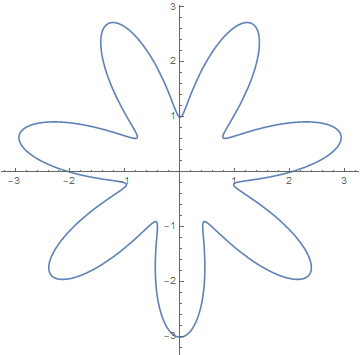
\includegraphics[scale=0.8]{image1.png}
		\end{figure}
		
		It makes a fun flower-looking thing! Also, there are seven spokes coming from the $\sin(7t)$ term.
		
		\item Sketch the curve $\gamma$ and the vector field $f$ on the same graph.
		
		\codeword{vtfield = VectorPlot[{Cos[x], Sin[y]}, {x, -3, 3}, {y, -3, 3}]}
		
		\codeword{gamma = ParametricPlot[{(2 + Sin[7 t]) Cos[t], (2 + Sin[7 t]) Sin[t]}, {t, 0, 2 Pi}]}
		
		\codeword{Show[gamma, vtfield, PlotRange -> All]}
		
		Sets up plotting the vector field and curve $\gamma$ on on the same graph, which produces the following figure:
		
		\begin{figure}[H]
		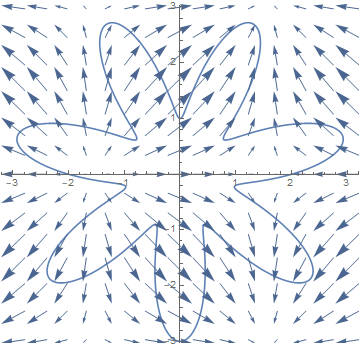
\includegraphics[scale=0.7]{image2.png}
		\end{figure}
		
		\item What is the Polya vector field of $f$?
		
		\[f(z)=\cos(x)+i\sin(y) \implies \overline{f}(z)=\cos(x)-i\sin(y)\]
		
		\item Find an approximation for the complex integral $\int_{\gamma}\overline{f}(z)dz.$
		
		\codeword{n = 100}
		
		\codeword{t[k_] := 2 *Pi* k/n}
		
		\codeword{z[k_] := (2 + Sin[7 t[k]]) Cos[t[k]] + I (2 + Sin[7 t[k]]) Sin[t[k]]}
		
		\codeword{f[z_] := Cos[Re[z]] - I Sin[Im[z]]}
		
		\codeword{N[Sum[f[z[k]]*(z[k + 1] - z[k]), {k, 0, n - 1}]]}
		
		Output: \codeword{0.0714602 + 5.91499 I}
		
		This code mimics the provided Mathematica guide by approximating the integral with 100 sample points along $\gamma$, being sure to use $\overline{f}$ instead of $f$.
		
		\item Find an approximation for the work done by $f$ along $\gamma$, and the flux of $f$ across $\gamma$.
		
		We know 
		\[W[f,\gamma]+iF[f,\gamma]=\int_{\gamma}\overline{f}(z)\ dz\approx\ 0.0714602 + i 5.91499 \]
		\[\implies W[f,\gamma]\approx\ 0.0714602 \text{ and } F[f,\gamma]\approx\ 5.91499 \]
	\end{enumerate}
\end{enumerate}

% ---------------------------------------------------
% Anything after the \end{document} will be ignored by the typesetting.
% ----------------------------------------------------

\end{document}

